\documentclass[12pt,a4paper]{article}
\usepackage[utf8]{inputenc}
\usepackage[spanish]{babel}
\usepackage{amsmath}
\usepackage{amsfonts}
\usepackage{amssymb}
\usepackage{graphicx}
\usepackage{geometry}
\usepackage{booktabs}
\usepackage{array}
\usepackage{multirow}
\usepackage{float}
\usepackage{subcaption}
\usepackage{listings}
\usepackage{xcolor}
\usepackage{hyperref}

% Configuración para listings (código Python)
\lstset{
    language=Python,
    basicstyle=\ttfamily\footnotesize,
    keywordstyle=\color{blue}\bfseries,
    commentstyle=\color{green!60!black},
    stringstyle=\color{red},
    numbers=left,
    numberstyle=\tiny\color{gray},
    stepnumber=1,
    numbersep=5pt,
    showspaces=false,
    showstringspaces=false,
    showtabs=false,
    frame=single,
    tabsize=4,
    captionpos=b,
    breaklines=true,
    breakatwhitespace=false,
    backgroundcolor=\color{gray!10}
}

\geometry{margin=2.5cm}

\title{\textbf{Examen: Statistical Learning}}
\author{Andrés Proaño}
\date{\today}

\begin{document}

\maketitle

\section{Ejercicio 1: Boston Housing Datasets}

Se trabajará con el dataset Boston Housing que contiene información sobre viviendas en Boston, Massachusetts. El objetivo es predecir el valor mediano de las viviendas.

El dataset contiene las siguientes variables:
\begin{itemize}
\item CRIM     per capita crime rate by town
\item ZN       proportion of residential land zoned for lots over 25,000 sq. ft.
\item INDUS    proportion of non-retail business acres per town
\item CHAS     Charles River dummy variable (1 if tract bounds river; 0 otherwise)
\item  AGE      proportion of owner-occupied units built prior to 1940
\item  DIS      weighted distances to five Boston employment centres
\item  RAD      index of accessibility to radial highways
\item  TAX      full-value property-tax rate per \$10,000
\item  PTRATIO  pupil-teacher ratio by town
\item  B        $1000(Bk - 0.63)^2$ where Bk is the proportion of blacks by town
\item  LSTAT    porcentaje de población de bajo estatus
\item  MEDV     Median value of owner-occupied homes in \$1000's
\end{itemize}


\subsection{Base de Datos}

Se utilizó el conjunto de datos Boston Housing disponible en la Universidad de Toronto con fines educativos.

\begin{lstlisting}[language=Python, frame=single, basicstyle=\ttfamily\small, breaklines=true]
data_url = "http://lib.stat.cmu.edu/datasets/boston"
raw_df = pd.read_csv(data_url, sep="\s+", skiprows=22, header=None)
data = np.hstack([raw_df.values[::2, :], raw_df.values[1::2, :2]])
target = raw_df.values[1::2, 2]
\end{lstlisting}

\subsection{Objetivo}

El objetivo es predecir el valor mediano de las viviendas comparando diferentes modelos y sus rendimientos.

\subsection{Tareas Requeridas}

\subsubsection{Implementación de Modelos}

Antes de realizar los diferentes modelos, vamos a buscar significancia dentro de las variables para evitar utilizar datos que no aporten al trabajo.

\begin{figure}[H]
\centering
% Primera fila
\begin{subfigure}[t]{0.24\textwidth}
    \centering
    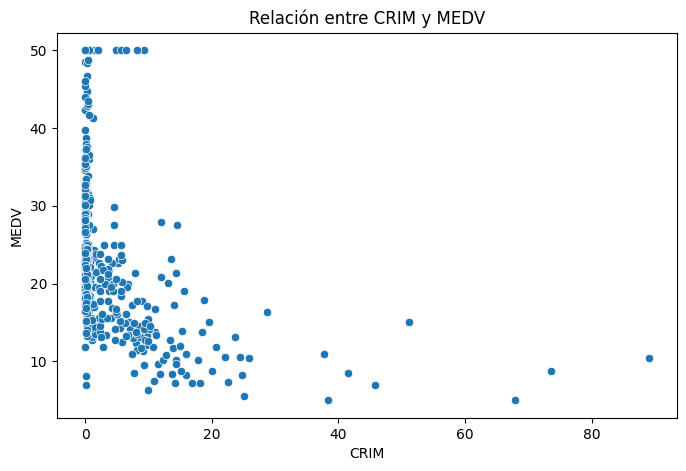
\includegraphics[width=\textwidth]{images/crim_medv.png}
    \caption{\footnotesize Tasa de criminalidad per cápita}
    \label{fig:modelo_crim}
\end{subfigure}
\hfill
\begin{subfigure}[t]{0.24\textwidth}
    \centering
    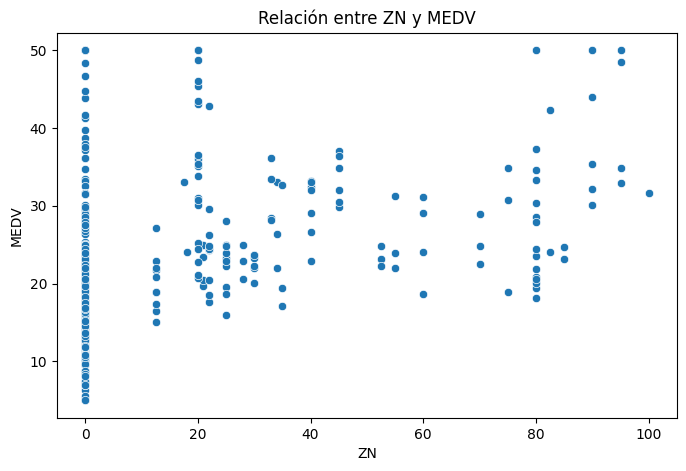
\includegraphics[width=\textwidth]{images/zn_medv.png}
    \caption{\footnotesize Proporción de terrenos residenciales}
    \label{fig:modelo_zn}
\end{subfigure}
\hfill
\begin{subfigure}[t]{0.24\textwidth}
    \centering
    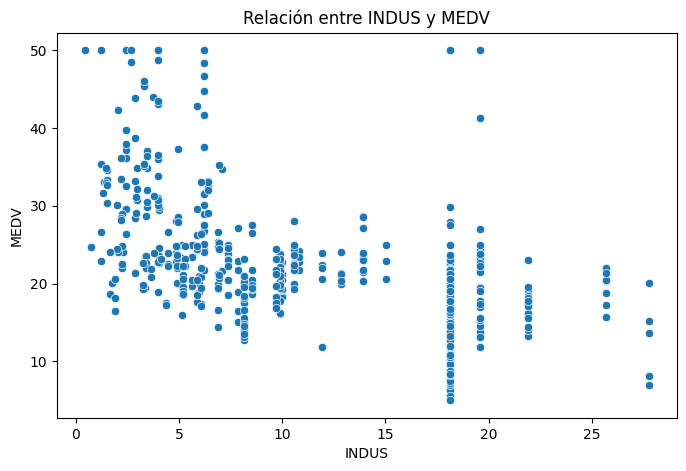
\includegraphics[width=\textwidth]{images/indus_medv.png}
    \caption{\footnotesize Proporción de terrenos industriales}
    \label{fig:modelo_indus}
\end{subfigure}
\hfill
\begin{subfigure}[t]{0.24\textwidth}
    \centering
    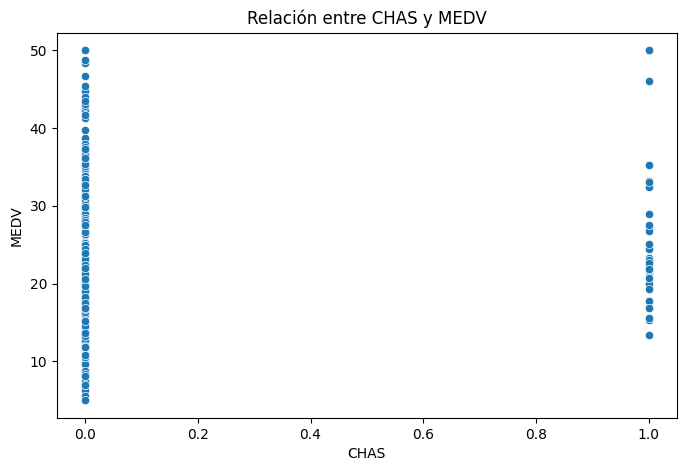
\includegraphics[width=\textwidth]{images/chas_medv.png}
    \caption{\footnotesize Variable Dummy del Río Charles}
    \label{fig:modelo_chas}
\end{subfigure}

\vspace{0.2cm}

% Segunda fila
\begin{subfigure}[t]{0.24\textwidth}
    \centering
    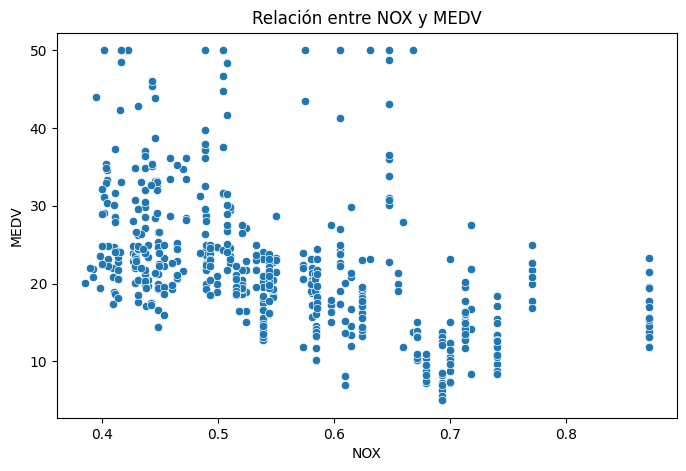
\includegraphics[width=\textwidth]{images/nox_medv.png}
    \caption{\footnotesize Concentración de Óxidos de Nitrógeno}
    \label{fig:modelo_nox}
\end{subfigure}
\hfill
\begin{subfigure}[t]{0.24\textwidth}
    \centering
    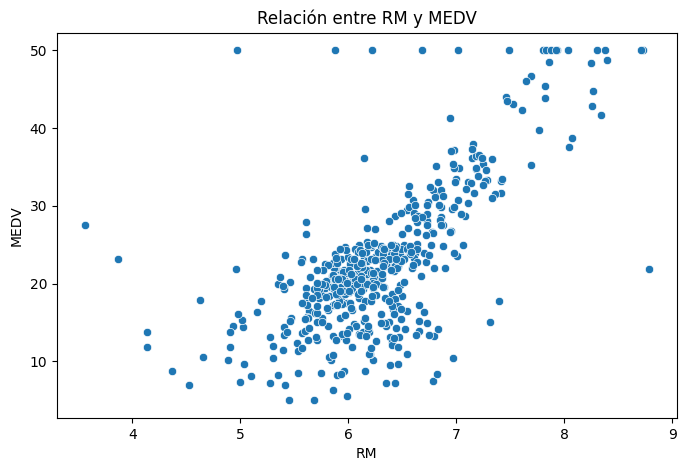
\includegraphics[width=\textwidth]{images/rm_medv.png}
    \caption{\footnotesize Número promedio de habitaciones}
    \label{fig:modelo_rm}
\end{subfigure}
\hfill
\begin{subfigure}[t]{0.24\textwidth}
    \centering
    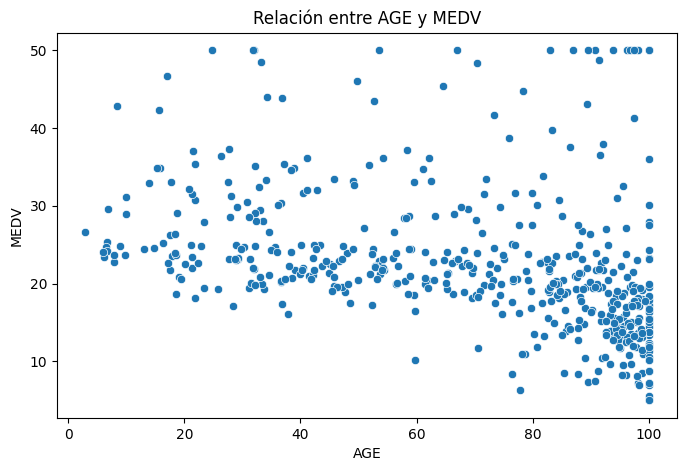
\includegraphics[width=\textwidth]{images/age_medv.png}
    \caption{\footnotesize Edad}
    \label{fig:modelo_age}
\end{subfigure}
\hfill
\begin{subfigure}[t]{0.24\textwidth}
    \centering
    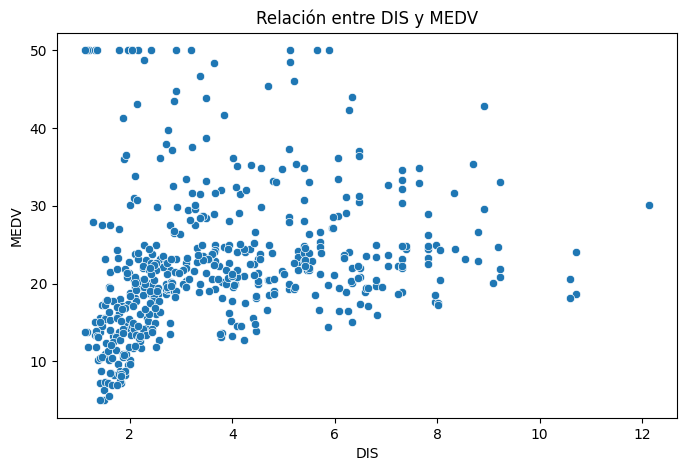
\includegraphics[width=\textwidth]{images/dis_medv.png}
    \caption{\footnotesize Distancia a centros de empleo}
    \label{fig:modelo_dis}
\end{subfigure}

\vspace{0.2cm}

\begin{subfigure}[t]{0.24\textwidth}
    \centering
    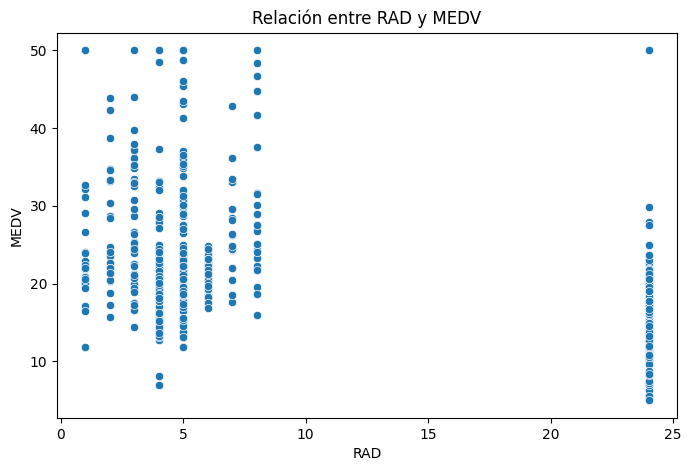
\includegraphics[width=\textwidth]{images/rad_medv.png}
    \caption{\footnotesize Accesibilidad a autopistas radiales}
    \label{fig:modelo_rad}
\end{subfigure}
\hfill
\begin{subfigure}[t]{0.24\textwidth}
    \centering
    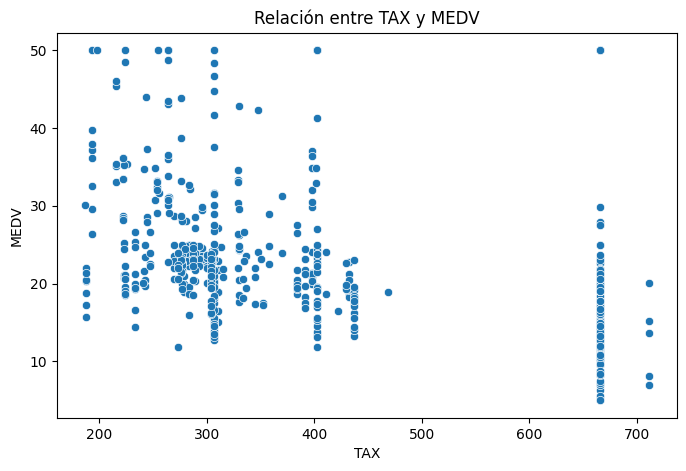
\includegraphics[width=\textwidth]{images/tax_medv.png}
    \caption{\footnotesize Tasa de impuesto predial}
    \label{fig:modelo_tax}
\end{subfigure}
\hfill
\begin{subfigure}[t]{0.24\textwidth}
    \centering
    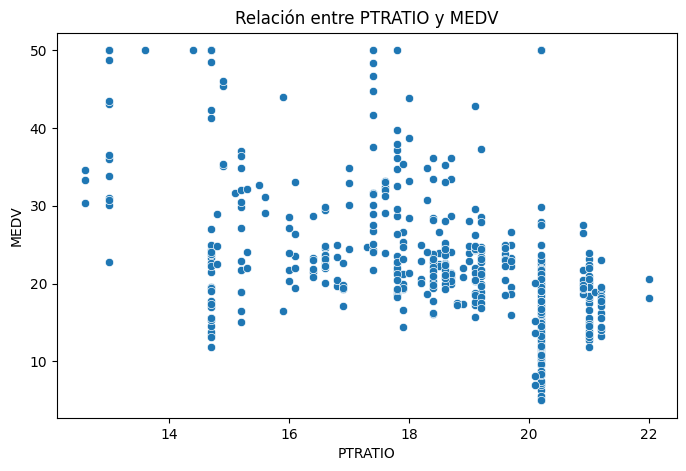
\includegraphics[width=\textwidth]{images/ptratio_medv.png}
    \caption{\footnotesize Relación de Población por Área}
    \label{fig:modelo_ptratio}
\end{subfigure}
\hfill
\begin{subfigure}[t]{0.24\textwidth}
    \centering
    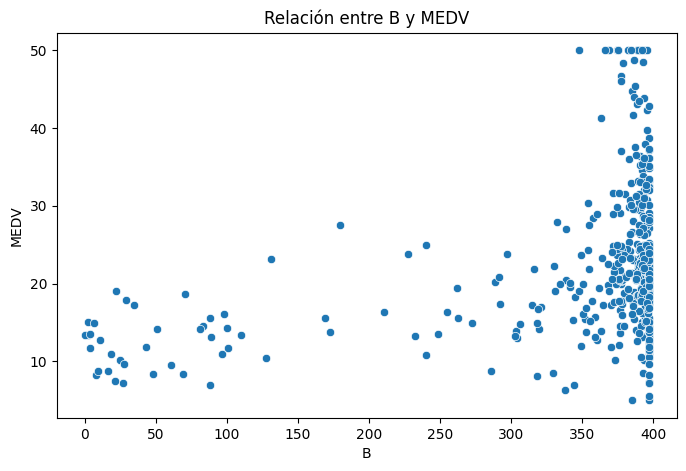
\includegraphics[width=\textwidth]{images/b_medv.png}
    \caption{\footnotesize Proporción de población negra}
    \label{fig:modelo_b}
\end{subfigure}

\vspace{0.2cm}

\begin{subfigure}[t]{0.24\textwidth}
    \centering
    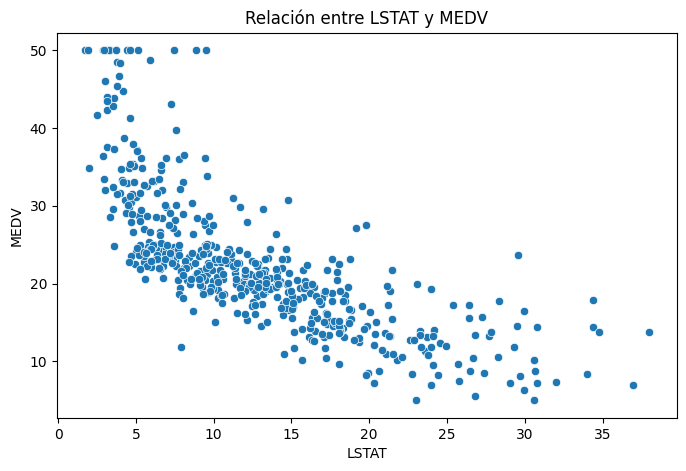
\includegraphics[width=\textwidth]{images/lstat_medv.png}
    \caption{\footnotesize Porcentaje de población de bajo estatus}
    \label{fig:modelo_lstat}
\end{subfigure}

\caption{Distribución de variables por Valor Mediano de Viviendas}
\label{fig:distribucion_variables}
\end{figure}

Como podemos observar, todas las variables son significativas al momento de tomar en cuenta el precio de la casa. Por lo tanto, se utilizarán todas las variables para los diferentes modelos.

\vspace{0.5cm}

\subsection{Modelo lineal Gaussiano (MLG)}

Para realizar el MLG utilizamos el siguiente código:

\begin{lstlisting}[language=Python, frame=single, basicstyle=\ttfamily\small, breaklines=true]
splitter = ShuffleSplit(n_splits=50, test_size=0.3, random_state=42)

mae_scores_mlg, rmse_scores_mlg = [], []

for train_index, test_index in splitter.split(x):
    X_train, X_test = x[train_index], x[test_index]
    y_train, y_test = y[train_index], y[test_index]

    X_train_sm = sm.add_constant(X_train, has_constant='add')
    X_test_sm = sm.add_constant(X_test, has_constant='add')

    model_gaussian = sm.GLM(y_train, X_train_sm, family=sm.families.Gaussian())
    fitted = model_gaussian.fit()

    y_pred_gaussian = fitted.predict(X_test_sm)

    mae_scores_mlg.append(mean_absolute_error(y_test, y_pred_gaussian))
    rmse_scores_mlg.append(mean_squared_error(y_test, y_pred_gaussian) ** 0.5)


mae_median = np.median(mae_scores_mlg)
mae_std = np.std(mae_scores_mlg, ddof=1)
rmse_median = np.median(rmse_scores_mlg)
rmse_std = np.std(rmse_scores_mlg, ddof=1)

print(f"Gaussian Model MAE: {mae_median:.2f} +/- {mae_std:.2f}")
print(f"Gaussian Model RMSE: {rmse_median:.2f} +/- {rmse_std:.2f}")
\end{lstlisting}

Obteniendo los siguientes resultados:

\vspace{0.3cm}

\begin{table}[H]
\centering
\caption{Resultados del Modelo Lineal Gaussiano}\label{tab:regresion_resultados}
\begin{tabular}{lcc}
\toprule
\textbf{Métrica} & \textbf{Valor} \\
\midrule
MAE & 3.39 +- 0.22  \\
RMSE & 4.91 ± 0.45  \\
\bottomrule
\end{tabular}
\end{table}

\subsubsection{Interpretación de los resultados}

Los resultados del modelo lineal Gaussiano indica que la diferencia entre los valores reales de MEDV y los valores estimados por el modelo es de 3.39 mil dólares, con una variabilidad moderadamente baja.
El RMSE, al ser más sensible a errores grandes, indica que las desviaciones cuadráticas promedio equivalen a unos 4.91 mil dólares, lo que sugiere que existen algunos errores más grandes, aunque no dominantes.

\subsection{Modelo lineal con regularización Elastic Net}

Para la realización utilizamos el siguiente código:

\begin{lstlisting}[language=Python, frame=single, basicstyle=\ttfamily\small, breaklines=true]
param_grid = {
    "elastic__alpha": [0.001, 0.01, 0.1, 1, 10],
    "elastic__l1_ratio": [0.1, 0.3, 0.5, 0.7, 0.9, 0.99],
}

pipeline = Pipeline([
    ("scaler", StandardScaler()),
    ("elastic", ElasticNet(max_iter=5000, random_state=42))
])

inner_cv = KFold(n_splits=7, shuffle=True, random_state=42)
splitter = ShuffleSplit(n_splits=50, test_size=0.3, random_state=42)

mae_scores, rmse_scores = [], []

for train_idx, test_idx in splitter.split(X_sm.values):
    X_train, X_test = X_sm.iloc[train_idx], X_sm.iloc[test_idx]
    y_train, y_test = y[train_idx], y[test_idx]

    grid = GridSearchCV(
        pipeline,
        param_grid,
        scoring="neg_mean_squared_error",
        cv=inner_cv,
        n_jobs=-1
    )
    grid.fit(X_train, y_train)

    y_pred = grid.predict(X_test)

    mae_scores.append(mean_absolute_error(y_test, y_pred))
    rmse_scores.append(mean_squared_error(y_test, y_pred) ** 0.5)

mae_median = np.median(mae_scores)
mae_std = np.std(mae_scores, ddof=1)
rmse_median = np.median(rmse_scores)
rmse_std = np.std(rmse_scores, ddof=1)

print(f"Elastic Net MAE: {mae_median:.2f} +/- {mae_std:.2f}")
print(f"Elastic Net RMSE: {rmse_median:.2f} +/- {rmse_std:.2f}")
\end{lstlisting}

Obteniendo los siguientes resultados:

\begin{table}[H]
\centering
\caption{Métricas de Rendimiento del Elastic Net}\label{tab:elastic_net_resultados}
\begin{tabular}{lc}
\toprule
\textbf{Métrica} & \textbf{Valor} \\
\midrule
MAE & 3.36 ± 0.22 \\
RMSE & 4.90 ± 0.47 \\
\bottomrule
\end{tabular}
\end{table}

\subsubsection{Interpretación de Resultados}
El modelo de regresión Elastic Net, tras realizar 50 particiones aleatorias de validación cruzada, arroja un error absoluto medio de 3.36 mil dólares y un error cuadrático medio de 4.90 mil dólares sobre la variable objetivo MEDV.
La dispersión de las métricas (± 0.22 y ± 0.47 respectivamente) es relativamente baja, lo que indica que el modelo mantiene un rendimiento estable ante diferentes divisiones de entrenamiento y prueba.
\vspace{1cm}

\subsection{Modelo lineal con componentes principales (PCA)}

\begin{lstlisting}[language=Python, frame=single, basicstyle=\ttfamily\small, breaklines=true]
pipeline = Pipeline([
    ("scaler", StandardScaler()),
    ("pca", PCA()),
    ("linreg", LinearRegression())
])

param_grid = {
    "pca__n_components": [5, 7, 9, 11, None]
}

inner_cv = KFold(n_splits=7, shuffle=True, random_state=42)
splitter = ShuffleSplit(n_splits=50, test_size=0.3, random_state=42)

mae_scores, rmse_scores = [], []

for train_idx, test_idx in splitter.split(X_sm.values):
    X_train, X_test = X_sm.iloc[train_idx], X_sm.iloc[test_idx]
    y_train, y_test = y[train_idx], y[test_idx]

    grid = GridSearchCV(
        pipeline,
        param_grid,
        scoring="neg_mean_squared_error",
        cv=inner_cv,
        n_jobs=-1
    )
    grid.fit(X_train, y_train)

    y_pred = grid.predict(X_test)

    mae_scores.append(mean_absolute_error(y_test, y_pred))
    rmse_scores.append(mean_squared_error(y_test, y_pred)**0.5)

mae_median = np.median(mae_scores)
mae_std = np.std(mae_scores, ddof=1)
rmse_median = np.median(rmse_scores)
rmse_std = np.std(rmse_scores, ddof=1)

print(f"PCA + LR MAE: {mae_median:.2f} +/- {mae_std:.2f}")
print(f"PCA + LR RMSE: {rmse_median:.2f} +/- {rmse_std:.2f}")
\end{lstlisting}

Obteniendo los siguientes resultados:

\begin{table}[H]
\centering
\caption{Métricas de Rendimiento del PCA}\label{tab:pca_resultados}
\begin{tabular}{lc}
\toprule
\textbf{Métrica} & \textbf{Valor} \\
\midrule
MAE & 3.39 ± 0.22 \\
RMSE & 4.91 ± 0.47  \\
\bottomrule
\end{tabular}
\end{table}

\subsubsection{Interpretación de Resultados}

Esto significa que, en promedio, el modelo comete un error absoluto de aproximadamente 3.4 mil dólares en la predicción de MEDV y un error cuadrático medio de unos 4.9 mil dólares. La baja desviación estándar de ambas métricas indica que el comportamiento es estable frente a diferentes particiones de validación cruzada.
\vspace{1cm}

\subsection{Maquinas de Vector de Soporte para Regresión (SVR)}

Para realizar el SVR utilizamos el siguiente código:

\begin{lstlisting}[language=Python, frame=single, basicstyle=\ttfamily\small, breaklines=true]
svr_pipeline = Pipeline([
    ("scaler", StandardScaler()),
    ("svr", SVR())
])

param_grid = {
    "svr__kernel": ["linear", "rbf"],
    "svr__C": [0.1, 1, 10],
    "svr__epsilon": [0.01, 0.1, 1],
    "svr__gamma": ["scale", "auto"]  # solo se usa cuando kernel='rbf'
}

inner_cv = KFold(n_splits=7, shuffle=True, random_state=42)
splitter = ShuffleSplit(n_splits=50, test_size=0.3, random_state=42)

mae_scores, rmse_scores = [], []

for train_idx, test_idx in splitter.split(X_sm.values):
    X_train, X_test = X_sm.iloc[train_idx], X_sm.iloc[test_idx]
    y_train, y_test = y[train_idx], y[test_idx]

    grid = GridSearchCV(
        svr_pipeline,
        param_grid,
        scoring="neg_mean_squared_error",
        cv=inner_cv,
        n_jobs=-1
    )
    grid.fit(X_train, y_train)

    y_pred = grid.predict(X_test)

    mae_scores.append(mean_absolute_error(y_test, y_pred))
    rmse_scores.append(mean_squared_error(y_test, y_pred) ** 0.5)

mae_median = np.median(mae_scores)
mae_std = np.std(mae_scores, ddof=1)
rmse_median = np.median(rmse_scores)
rmse_std = np.std(rmse_scores, ddof=1)

print(f"SVR MAE:  {mae_median:.2f} +/- {mae_std:.2f}")
print(f"SVR RMSE: {rmse_median:.2f} +/- {rmse_std:.2f}")
\end{lstlisting}

Obteniendo los siguientes resultados:

\begin{table}[H]
\centering
\caption{Métricas de Rendimiento del Modelo SVR}\label{tab:svr_resultados}
\begin{tabular}{lc}
\toprule
\textbf{Métrica} & \textbf{Valor} \\
\midrule
MAE & 2.35 ± 0.25 \\
RMSE & 3.88 ± 0.61 \\
\bottomrule
\end{tabular}
\end{table}

\subsubsection{Interpretación de Resultados}

El modelo SVR presenta un error medio absoluto de 2.35 mil dólares y un error cuadrático medio de 3.88 mil dólares al predecir el valor medio de viviendas (MEDV).

La desviación estándar moderadamente baja de ambas métricas (± 0.25 y ± 0.61) indica que el desempeño del modelo es consistente y estable a lo largo de las múltiples particiones de validación cruzada.
\newpage

\subsection{Árbol de decisión para regresión}

Para realizar el Árbol de Decisión para regresión utilizamos el siguiente código:

\begin{lstlisting}[language=Python, frame=single, basicstyle=\ttfamily\small, breaklines=true]
dtree = DecisionTreeRegressor(random_state=42)

param_grid = {
    "max_depth": [3, 5, 7, 9, None],
    "min_samples_split": [2, 5, 10],
    "min_samples_leaf": [1, 2, 5]
}

inner_cv = KFold(n_splits=7, shuffle=True, random_state=42)
splitter = ShuffleSplit(n_splits=50, test_size=0.3, random_state=42)

mae_scores, rmse_scores = [], []

for train_idx, test_idx in splitter.split(X_sm.values):
    X_train, X_test = X_sm.iloc[train_idx], X_sm.iloc[test_idx]
    y_train, y_test = y[train_idx], y[test_idx]

    grid = GridSearchCV(
        dtree,
        param_grid,
        scoring="neg_mean_squared_error",
        cv=inner_cv,
        n_jobs=-1
    )
    grid.fit(X_train, y_train)

    y_pred = grid.predict(X_test)

    mae_scores.append(mean_absolute_error(y_test, y_pred))
    rmse_scores.append(mean_squared_error(y_test, y_pred) ** 0.5)

mae_median = np.median(mae_scores)
mae_std = np.std(mae_scores, ddof=1)
rmse_median = np.median(rmse_scores)
rmse_std = np.std(rmse_scores, ddof=1)

print(f"Decision Tree MAE:  {mae_median:.2f} +/- {mae_std:.2f}")
print(f"Decision Tree RMSE: {rmse_median:.2f} +/- {rmse_std:.2f}")
\end{lstlisting}

Con este código obtenemos los siguientes resultados:

\begin{table}[H]
\centering
\caption{Métricas de Rendimiento del Árbol de Decisión para Regresión}\label{tab:dtree_resultados}
\begin{tabular}{lc}
\toprule
\textbf{Métrica} & \textbf{Valor} \\
\midrule
MAE & 2.97 ± 0.42 \\
RMSE & 4.53 ± 0.94 \\
\bottomrule
\end{tabular}
\end{table}

\subsubsection{Interpretación de Resultados}

El modelo de árbol de decisión presenta un error absoluto medio de 2.97 mil dólares y un error cuadrático medio de 4.53 mil dólares al predecir el valor medio de viviendas (MEDV).

Las desviaciones estándar (± 0.42 para MAE y ± 0.94 para RMSE) son moderadas, lo que indica que el rendimiento varía entre splits, pero no de manera incontrolada.

\section{Ejercicio 2: Stroke Prediction Dataset}

Se trabajará con el dataset Stroke Prediction que contiene información sobre pacientes y la predicción de accidentes cerebrovasculares.

El dataset contiene las siguientes variables:
\begin{itemize}
\item id     Unique id
\item gender       Gender of the patient
\item age          Age of the patient
\item hypertension Hypertension status 
\item heart_disease Heart disease status 
\item ever_married Has the patient being married 
\item work_type    Type of work 
\item residence_type Type of residence 
\item avg_glucose_level Average glucose level
\item bmi          Body mass index
\item smoking_status Smoking status
\item stroke       Stroke status 
\end{itemize}

\subsection{Base de Datos}

Se utilizó el conjunto de datos Stroke Prediction disponible en la siguiente URL https://www.kaggle.com/datasets/fedesoriano/stroke-prediction-dataset.

\begin{lstlisting}[language=Python, frame=single, basicstyle=\ttfamily\small, breaklines=true]
# Install dependencies as needed:
# pip install kagglehub[pandas-datasets]
import kagglehub
from kagglehub import KaggleDatasetAdapter

# Load the latest version
df = kagglehub.dataset_load(
  KaggleDatasetAdapter.PANDAS,
  "fedesoriano/stroke-prediction-dataset",
  "healthcare-dataset-stroke-data.csv",
  # Provide any additional arguments like 
  # sql_query or pandas_kwargs. See the 
  # documenation for more information:
  # https://github.com/Kaggle/kagglehub/blob/main/README.md#kaggledatasetadapterpandas
)

print("First 5 records:", df.head())
\end{lstlisting}

\subsection{Pregunta de Investigación}

¿Cuáles son los principales factores de riesgo para accidente cerebrovascular y cómo podemos predecir
eficientemente pacientes en riesgo?

\subsection{Tareas Requeridas}

\subsubsection{Implementación de Modelos}

\end{document}